\documentclass[11pt, a4paper]{article}


\usepackage[utf8]{inputenc}
\usepackage[english]{babel}
\usepackage[T1]{fontenc}
\usepackage{geometry}
\geometry{a4paper, margin=1in}


\usepackage{amsmath}
\usepackage{amssymb}
\usepackage{graphicx} 
\usepackage{booktabs}
\usepackage{tikz}


\usepackage{xcolor} 
\usepackage{hyperref}
\hypersetup{
	colorlinks=true,
	linkcolor=blue,
	urlcolor=blue,
	citecolor=blue,
	pdftitle={A Layered Conceptual Framework: From Quantum Duality to Meta-Reflection in a Holographic Universe, Unified by the Universal Binary Scale (UBS)},
	pdfauthor={José Arturo Ornelas Brand}
}
\usepackage{bookmark} 
\usepackage{enumitem} 


\title{\textbf{A Layered Conceptual Framework: From Quantum Duality to Meta-Reflection in a Holographic Universe, Unified by the Universal Binary Scale (UBS)}}
\author{
	José Arturo Ornelas Brand \\
	\textit{Independent Researcher} \\
	\href{mailto:arturoornelas62@gmail.com}{\texttt{arturoornelas62@gmail.com}}
}
\date{\today}


\begin{document}
	
	\maketitle
	\tableofcontents
	\newpage
	
	\begin{abstract}
		This paper introduces a novel layered conceptual framework that describes the evolution of reality from fundamental quantum dualities to a meta-reflective, holographic universe. Comprising nine progressive layers, the framework integrates geometric emergence, dynamic interactions, information entropy, and recursive cycles to explain the multiplication of conceptual units and the unification of measurable phenomena. Complementing this, the Universal Binary Scale (UBS) serves as a unifying metric, quantifying all elements in bits of information entropy, drawing from Shannon's theory, Wheeler's "It from Bit," and holographic principles. The framework posits that opposites and complexity arise through iterative duplication, limited by entropy bounds, providing an intuitive model for cosmic evolution. We formalize this with axioms, derive implications for interdisciplinary applications, and demonstrate algorithmic implementations for simulation and optimization.
	\end{abstract}
	
	\section{Introduction}
	
	In the quest for a unified understanding of reality, theoretical physics and information science have converged on principles where the universe emerges from fundamental bits of information, as encapsulated in John Wheeler's seminal idea of "It from Bit" \cite{wheeler1990}. This paper builds upon such foundations to propose a comprehensive layered conceptual framework that traces the progression from basic quantum dualities to a meta-reflective holographic cosmos. At its core, the framework consists of nine interconnected layers, each representing a stage in the conceptual evolution: starting with an indivisible point embodying existence/non-existence duality (inspired by qubits), advancing through geometric and dynamic structures, and culminating in recursive cycles that explain self-sustaining multiplication and complexity.
	
	Complementing this layered progression is the Universal Binary Scale (UBS), a metric that unifies measurable concepts across domains by expressing them in bits of entropy. Drawing from Claude Shannon's information theory \cite{shannon1948}, Jacob Bekenstein's entropy bounds \cite{bekenstein1973}, and recent holographic dualities \cite{maldacena1999}, UBS quantifies ranges, precisions, and uncertainties, providing a rigorous tool to measure and integrate the framework's elements.
	
	This synthesis addresses key questions: Why does a fundamental point multiply into lines and volumes? How does entropy limit and drive universal evolution? And how can such principles inform practical algorithms for simulation and optimization? The motivation stems from the need for an intuitive "basic form" to describe cosmic evolution, as highlighted in discussions of holographic reality \cite{bousso2002}. Our framework offers this by blending philosophical ontology with computational rigor, enabling applications in quantum simulation, artificial intelligence self-improvement, and interdisciplinary unification. We begin by outlining the foundational axioms, then detail the nine layers, and conclude with algorithmic implementations and future directions.
	
	\section{Foundational Axioms}
	The framework is grounded in a set of axioms that formalize the emergence of complexity from fundamental dualities. These axioms draw from principles in information theory, quantum mechanics, holographic duality, and Emergence Theory (e.g., its code-theoretic axiom and Euclid's postulates for geometric foundations \cite{qgr2023}), providing a deductive basis for the layered progression. We present six core axioms, with a new one added for code-theoretic discretization to enhance foundational rigor, refined to integrate binary scales, recursive elements, fractal self-similarity, relational dynamics, and computational principles (e.g., least action in code syntax), ensuring consistency with the Universal Binary Scale (UBS) and updated analogies (e.g., quasicrystals for geometric emergence \cite{qgr2023}, "It from Qubit" for entanglement \cite{li2024}, entropic gravity \cite{verlinde2010}). UBS is standardized as \( \mathcal{UBS}(X) = \log_2 (X / X_0) + S(X) \), where \( X_0 \) is a Planck-scale unit and \( S(X) \) is the associated entropy, bounded holographically to prevent divergence.
	
	\begin{enumerate}
		\item \textbf{Axiom of Initial Duality (Quantum Binary Foundation)}: All conceptual entities originate from an indivisible unit embodying a fundamental duality of existence (1) and non-existence (0), equivalent to a qubit state \( |\psi\rangle = \alpha |0\rangle + \beta |1\rangle \) with \( |\alpha|^2 + |\beta|^2 = 1 \). This duality implies the emergence of time as a measure of transitions between states and enables relational quantum dynamics, where states are defined by interactions \cite{rovelli1996}. Quantified in bits via UBS as \( \mathcal{UBS}(D) = H(\rho) \), where \( H(\rho) = -\text{Tr}(\rho \log_2 \rho) \) is the von Neumann entropy, linking to "It from Qubit" for entanglement emergence and Fibonacci chains isomorphic to binary strings in Emergence Theory \cite{li2024,qgr2023}.
		
		\item \textbf{Axiom of Evolutionary Multiplication}: Dual states multiply through iterative operations (sum/subtraction), generating extensions and emergent properties with fractal self-similarity. Complexity scales as \( 2^n \) for \( n \) iterations, with opposites arising at thresholds (e.g., \( b_i \neq b_{i+1} \)), mirroring fractal cosmologies \cite{notale1993}. This explains the progression from points to lines, formalized as \( \mathcal{UBS}(M) = n + S(n) \), where \( S(n) \) bounds iterations entropically, reflecting recursive syntax choices in code-theoretic models \cite{qgr2023}.
		
		\item \textbf{Axiom of Geometric Emergence}: Connections of dual elements form multidimensional structures (lines to triangles to tetrahedrons), where higher dimensions enclose information bounded by lower ones, akin to holographic principles and quasicrystal tilings in Emergence Theory, building on Euclid's postulate of straight lines between points for flat 1D spaces extended to higher dimensions \cite{qgr2023}. Volume \( V \) is unified in UBS as \( \mathcal{UBS}(V) = \log_2 (V / l_P^3) + S(V) \), with \( S(V) \) as Bekenstein entropy \cite{bekenstein1973} and \( l_P \) the Planck length.
		
		\item \textbf{Axiom of Entropic Dynamics}: Interactions produce energy and information, governed by entropy as a universal limiter, with dynamics emerging from information gradients as in entropic gravity \cite{verlinde2010}. Dynamics are quantified as \( \mathcal{UBS}(E) = \log_2 (E / E_P) + S(E) \), where \( S(E) = k \ln 2 \cdot H \), ensuring conservation and emergence of opposites in quantum and classical regimes, aligned with principles of least computational action in code-theoretic frameworks \cite{qgr2023}.
		
		\item \textbf{Axiom of Meta-Recursive Cycles}: The system is self-referential, with higher layers retroactively influencing lower ones through observation-induced collapses, creating recursive cycles that drive continuous multiplication and potential multiversal branching \cite{notale1993}. This is bounded by holographic entropy \( S \leq A / (4 l_P^2 \ln 2) \), unifying the framework in a closed loop with feedback via viewing vectors in geometric primitives and non-local empire waves in quasicrystals \cite{qgr2023}.
		
		\item \textbf{Axiom of Code-Theoretic Discretization (New)}: Reality is fundamentally code-theoretic, consisting of a finite set of object types (e.g., binary dualities) with syntactical rules and degrees of freedom, discretizing spacetime into a quasicrystalline spin network where phason quasiparticles propagate according to non-deterministic syntax, enabling emergent geometry and self-organization \cite{qgr2023}. This is quantified via UBS as \( \mathcal{UBS}(C) = \log_2 (|Code| / |Base|) + S_{syntax} \), where \( |Code| \) is the code complexity, \( |Base| \) is the fundamental unit count, and \( S_{syntax} \) is entropy from rule choices, bounded by holographic non-locality to support recursive and holographic principles.
	\end{enumerate}
	These axioms serve as the deductive core, from which the layered structure is derived. They ensure that the framework is not merely descriptive but capable of generating testable predictions and algorithmic implementations, such as simulations of quasicrystalline codes for emergent phenomena.
	
	\section{The Universal Binary Scale (UBS): A Unifying Metric}
	The Universal Binary Scale (UBS) is a novel metric designed to quantify all elements of the framework in bits of information entropy, providing a unified measure across scales from quantum dualities to cosmic evolution. Drawing from Claude Shannon's information theory \cite{shannon1948}, John Wheeler's "It from Bit" paradigm \cite{wheeler1990}, Jacob Bekenstein's entropy bounds \cite{bekenstein1973}, and recent advancements in holographic principles \cite{bousso2002,maldacena1999}, UBS expresses measurable phenomena (e.g., lengths, energies, volumes) in logarithmic binary units augmented by entropy terms. This update incorporates fractal self-similarity from scale-free informational matrices and computational holography frameworks, aligning with Emergence Theory's code-theoretic discretization and fractal expansions in universal information theories \cite{qgr2023,notale1993}. UBS addresses key challenges: unifying disparate scales, bounding complexity via holography, and enabling computational simulations, ensuring coherence with the six foundational axioms and the nine conceptual layers.
	
	\subsection{Definition and Standardization}
	UBS standardizes quantification as:
	\[
	\mathcal{UBS}(X) = \log_2 \left( \frac{X}{X_0} \right) + S(X),
	\]
	where:
	\begin{itemize}
		\item \( X \) is the measurable quantity (e.g., length, energy, volume).
		\item \( X_0 \) is the fundamental Planck-scale unit (e.g., \( l_P \) for length, \( E_P \) for energy).
		\item \( S(X) \) is the associated entropy (e.g., Shannon entropy \( H = -\sum p_i \log_2 p_i \), von Neumann entropy \( H(\rho) = -\text{Tr}(\rho \log_2 \rho) \), or Bekenstein-Hawking entropy \( S = \frac{A}{4 l_P^2 \ln 2} \)), ensuring holographic bounds to prevent informational divergence \cite{bekenstein1973,bousso2002}.
	\end{itemize}
	This form captures both the scale (logarithmic term for precision/range) and uncertainty (entropy term), reflecting the holographic principle where information is surface-encoded \cite{maldacena1999}. Special cases, such as pure entropy measures in foundational dualities (e.g., \( \mathcal{UBS}(D) = H(\rho) \) when the log term is zero for unit scales), align directly with Axiom 1.
	
	\subsection{Incorporating Fractal and Computational Aspects}
	To account for fractal self-similarity (per Axiom 2 and layers like 2 and 9, where iterative duplications scale recursively), UBS is extended for multi-scale phenomena:
	\[
	\mathcal{UBS}_{fractal}(X) = \log_2 \left( \frac{X}{X_0} \right) + S(X) + D_f \log_2 (scale),
	\]
	where \( D_f \) is the fractal dimension (e.g., Hausdorff dimension, typically 1 < \( D_f \) < 3 for quasicrystals as in Emergence Theory's non-periodic tilings \cite{qgr2023,levine1984}), and \( scale \) is the observational range (e.g., from Planck to cosmic horizon). This term integrates fractal entropy in holographic universes, where information expands nonlinearly, consistent with Axiom 3's geometric emergence and Layer 5's tetrahedral volumes \cite{notale1993}.
	
	For code-theoretic elements (aligning with the new Axiom 6 on discretization), UBS quantifies syntactic complexity:
	\[
	\mathcal{UBS}_{code}(C) = \log_2 (|Code| / |Base|) + S_{syntax},
	\]
	where \( |Code| \) is the total code length (e.g., in binary operations across layers), \( |Base| \) is the fundamental duality count, and \( S_{syntax} \) is entropy from rule variations, bounded by non-local holographic encoding \cite{qgr2023}. This directly supports Axiom 6's quantification of code complexity in quasicrystalline spin networks.
	
	\subsection{Global UBS for the Framework}
	Aggregating across layers for holistic unification (echoing Axiom 5's meta-recursive cycles and inter-layer fractal connections):
	\[
	\mathcal{UBS}_{total} = \sum_{i=1}^9 \mathcal{UBS}(L_i) + D_f \log_2 (scale) + S_{global},
	\]
	where \( S_{global} \) includes recursive entropy bounds (e.g., \( S \leq A / (4 l_P^2 \ln 2) \)), ensuring the entire system respects holographic limits (e.g., universe entropy ~ horizon area \cite{bousso2002}). This global form coheres with the layered progression, where each \( \mathcal{UBS}(L_i) \) (e.g., \( \mathcal{UBS}(V) \) in Layer 5) contributes additively, bounded by axioms like Entropic Dynamics (Axiom 4).
	
	\subsection{Integration with Axioms and Layers}
	UBS seamlessly integrates with the axioms: For instance, Axiom 1's duality entropy uses the pure \( S(X) \) form, while Axiom 3's geometric volumes add the scale log term, all bounded per Axiom 5. In the layers, UBS applications (e.g., \( \mathcal{UBS}(Cycle) \) in Layer 9 bounded holographically) reflect axiom-derived principles, with fractal extensions enhancing self-similar transitions (e.g., from Layer 2's lines to Layer 8's cosmic scales). This ensures no contradictions, as all formulations respect entropy conservation and holographic bounds, preventing infinite complexity in recursive cycles.
	
	\subsection{Applications and Implications}
	UBS enables interdisciplinary unification: e.g., in quantum computing, it optimizes qubit entropy per Layer 1; in cosmology, it bounds fractal multiverse branches per Layer 9 \cite{notale1993}. Testable via simulations (e.g., NetworkX for quasicrystal entropy in Layers 5-9) or black hole analogs \cite{bousso2002}. This metric posits that all reality is computable information, resolving scales in a holographic, fractal universe while maintaining coherence across the framework's deductive core and progressive layers.
	
	
	\section{The Nine Conceptual Layers}
	
	\subsection{Integrated Layer 1: Initial Duality (Qubit Base)}
	Definition: The foundational unit is an indivisible point representing the fundamental duality of existence (1) and non-existence (0), which originates time as a measure of probabilistic transitions between states. This point is analogous to a qubit in superposition, \( |\psi\rangle = \alpha |0\rangle + \beta |1\rangle \) with \( |\alpha|^2 + |\beta|^2 = 1 \), avoiding the Zeno paradox by treating time emergence as discrete, entropy-driven flips rather than continuous observation. This duality enables relational quantum dynamics, where states are defined by interactions rather than isolation \cite{rovelli1996}.
	
	Key Concepts: Existence (1), Non-Existence (0), Time (as transition metric), Qubit Superposition.
	
	Dualities: Existence-Non-Existence (encompassing state transitions).
	
	Physical/Quantum Analogy: Inspired by quantum fluctuations in vacuum energy, extended to qubits for superposition ambiguity, as in holographic duality models \cite{maldacena1999}. Parallels Emergence Theory's binary states at Planck-scale pixels \cite{qgr2023}. Explicitly links to "It from Qubit" for entanglement emergence \cite{li2024}.
	
	Transition: Iterative summation of such points, driven by duality resolution, evolves to lines, initiating geometric extension while preserving informational conservation.
	
	UBS Application: \( \mathcal{UBS}(D) = H(\rho) \), where \( H(\rho) = -\text{Tr}(\rho \log_2 \rho) \) is the von Neumann entropy, quantifying duality uncertainty in bits.
	
	Expansion: This layer establishes the binary foundation. For explicitness, consider a simple qubit model: a single spin-1/2 particle where measurement collapses the duality, producing measurable time intervals proportional to entropy resolution.
	
	\subsection{Integrated Layer 2: Line and Evolution}
	Definition: Through iterative summation (or subtraction as its dual), the initial point duplicates to form a line, introducing conceptual transformation and extension independent of pure time. This represents the first geometric emergence, where operations like addition create stable extensions from unstable dualities.
	
	Key Concepts: Line (as extended duality), Sum, Subtraction, Evolution (iterative change), Stability (fixed states post-operation).
	
	Dualities: Sum-Subtraction, Evolution-Stability.
	
	Physical/Quantum Analogy: Analogous to particle trajectories in 1D quantum mechanics or string theory's 1D vibratory modes \cite{greene1999}; in qubits, summation models initial entanglement pairs. Aligns with Emergence Theory's binary choices generating linear extensions in quasicrystal precursors \cite{qgr2023}. Lines exhibit self-similar extensions, mirroring fractal cosmologies where small-scale duplications scale up \cite{notale1993}.
	
	Transition: Properties such as direction and movement emerge from line attributes, preparing for unidimensional dynamics and eventual bidimensional connections.
	
	UBS Application: \( \mathcal{UBS}(L) = \log_2 (length / l_P) + S(L) \), where \( l_P \) is the Planck length and \( S(L) \) is line entropy.
	
	Expansion: The line forms via \( n \)-fold duplication: starting from one point, each iteration adds a dual point, scaling complexity as \( 2^n \) per axioms. This avoids infinite regress by bounding iterations with entropy, e.g., in simulations, lines represent quantum paths in Feynman diagrams.
	
	\subsection{Integrated Layer 3: Properties of the Line}
	Definition: The line generates derived attributes through inherent operations, integrating concepts like movement (change in position) and mathematical divisions/multiplications, all emerging from the underlying duality extensions.
	
	Key Concepts: Movement, Direction, Distance, Velocity, Division, Multiplication, Rest (absence of change), Separation, Proximity, Slowness (inverse velocity).
	
	Dualities: Movement-Rest (dynamics), Direction-Indirection (orientation), Distance-Proximity (separation), Velocity-Slowness (speed), Division-Multiplication (scaling).
	
	Physical/Quantum Analogy: Represents one-dimensional trajectories in classical mechanics or Hilbert space vectors in quantum mechanics; links to geometric quantum mechanics where lines encode phase space paths \cite{ashtekar2003}. Properties like direction emerge from non-local quantum relations, tying to emergent locality in amplituhedron models \cite{arkani2013}.
	
	Transition: Connections between lines form closed shapes like triangles, enabling bidimensional areas and angular relations.
	
	UBS Application: Velocity as \( \mathcal{UBS}(v) = \log_2 (v / v_P) + S(t) \), with Planck velocity \( v_P = c \) and \( S(t) \) as time-entropy.
	
	Expansion: These properties arise from interactions: e.g., velocity as rate of point duplication along the line, limited by relativistic bounds. In quantum terms, this layer models wavefunction propagation, with dualities reflecting uncertainty principles.
	
	\subsection{Integrated Layer 4: Triangle and Bidimensional Area}
	Definition: Three connected lines form a triangle, delimiting a bidimensional area and introducing angular relations, where the surface encodes information holographically bounded by its perimeter.
	
	Key Concepts: Triangle (closed 2D shape), Surface (enclosed area), Angular Relations (angles between lines), Bidimensional Void (unenclosed space).
	
	Dualities: Surface-Bidimensional Void, Angular Relations-Non-Angularity (flat vs. curved).
	
	Physical/Quantum Analogy: Corresponds to 2D planes in geometry or holographic encoding where information is projected onto surfaces \cite{bousso2002}; aligns with Emergence Theory's 2D projections in quasicrystal lattices \cite{qgr2023}. Surface entropy aligns with the generalized holographic principle \cite{bousso2002}.
	
	Transition: Adding a dimension via tetrahedral assembly leads to tridimensional volumes, with areas serving as bounding surfaces.
	
	UBS Application: \( \mathcal{UBS}(A) = \log_2 (A / l_P^2) + S(A) \), with holographic entropy bound \( S(A) \leq A / (4 l_P^2 \ln 2) \).
	
	Expansion: The triangle emerges from connecting three lines at vertices, each vertex resolving a duality. This layer introduces curvature concepts implicitly, e.g., non-Euclidean triangles in gravitational contexts.
	
	\subsection{Integrated Layer 5: Tetrahedron and Tridimensional Volume}
	Definition: Four triangles assemble into a tetrahedron, enclosing a tridimensional volume and defining spatial relations, where the volume's information is holographically encoded on its surface triangles.
	
	Key Concepts: Tetrahedron (minimal 3D polyhedron), Tridimensional Space (enclosed volume), Spatial Relations (distances/angles in 3D), Tridimensional Void (external space).
	
	Dualities: Tridimensional Space-Tridimensional Void, Spatial Relations-Non-Spatiality (localized vs. delocalized).
	
	Physical/Quantum Analogy: Central to Emergence Theory, where tetrahedrons are Planck-length 3D pixels in quasicrystals, with volume emerging from quantum entanglement on surfaces \cite{qgr2023}. Tetrahedrons form non-periodic tilings in Emergence Theory, enabling emergent curvature and gravity from code-like patterns \cite{qgr2023}.
	
	Transition: Interactions between multiple tetrahedrons generate dynamics, such as collisions or mergers.
	
	UBS Application: \( \mathcal{UBS}(V) = \log_2 (V / l_P^3) + S(V) \), bounded by holographic surface entropy.
	
	Expansion: Tetrahedrons tile space in non-periodic quasicrystals, modeling emergent spacetime. Example: In quantum gravity, volumes represent entanglement entropy regions.
	
	\subsection{Integrated Layer 6: Volumetric Interactions and Dynamics}
	Definition: Tetrahedral volumes interact in 3D space, producing forces, energy transfers, and motion, governed by conservation laws emerging from lower-layer dualities.
	
	Key Concepts: Dynamics (change via interaction), Interaction (volume contacts), Energy (stored potential), Statics (equilibrium), Isolation (non-interaction), Inertia (resistance to change).
	
	Dualities: Dynamics-Statics, Interaction-Isolation, Energy-Inertia.
	
	Physical/Quantum Analogy: Mirrors classical/relativistic mechanics or entropic gravity theories, where dynamics arise from information gradients \cite{verlinde2010}; quantumly, via entangled qubits in volumetric networks. Interactions produce emergent forces akin to gravity from information gradients \cite{verlinde2010}.
	
	Transition: These interactions encode and transmit information, leading to entropy measures in complex systems.
	
	UBS Application: \( \mathcal{UBS}(E) = \log_2 (E / E_P) + S(E) \), with Planck energy \( E_P \) and \( S(E) = k \ln 2 \cdot H \).
	
	Expansion: Integrate with Layer 5: e.g., tetrahedral tilings deform under interactions, simulating gravity as curvature in quasicrystals. Bounds prevent unbounded energy via entropy limits.
	
	\subsection{Integrated Layer 7: Information and Entropy (Quantum Complex Systems)}
	Definition: Volumetric dynamics produce information (encoded states) and entropy (measure of disorder/uncertainty), with transmission governed by quantum laws like no-cloning.
	
	Key Concepts: Information (bits of state), Entropy (disorder metric), Information Transmission (sharing), Order (low entropy), Quantum Information (superposed bits).
	
	Dualities: Information-Ignorance (known-unknown), Entropy-Order, Transmission-Blockage (defined as decoherence preventing perfect copy).
	
	Physical/Quantum Analogy: Draws from Shannon theory and quantum thermodynamics, with information conserved in unitary evolutions \cite{shannon1948}. Entropy bounds reflect holographic limits, as in black hole horizons encoding universal information \cite{bekenstein1973}.
	
	Transition: Accumulated information scales to holographic cosmic evolution.
	
	UBS Application: \( \mathcal{UBS}(H) = -\sum p_i \log_2 p_i + S_{bound} \), incorporating holographic bounds \( S \leq A / (4 l_P^2 \ln 2) \).
	
	Expansion: Entropy increases via interactions (second law analogy), but quantum bounds (e.g., Landauer limit) resolve uncertainties. Example: In qubits, entropy quantifies entanglement across systems.
	
	\subsection{Integrated Layer 8: Universe Evolution (Holographic)}
	Definition: Information and entropy drive cosmic expansion in a holographic framework, from initial dualities to large-scale structures, with spacetime emerging as a projection.
	
	Key Concepts: Holographic Evolution (projection from boundaries), Arrow of Time (entropy increase), Spacetime Emergence, Scale Unification (Planck to cosmic).
	
	Dualities: Expansion-Contraction, Cosmic Order-Disorder.
	
	Physical/Quantum Analogy: Based on AdS/CFT correspondence, where bulk gravity emerges from boundary quantum fields \cite{maldacena1999}; aligns with Emergence Theory's self-simulating quasicrystals \cite{qgr2023}. Evolution models a de Sitter-like universe emerging holographically from quantum fields \cite{afshordi2019}.
	
	Transition: Evolution culminates in meta-feedback loops, closing the system recursively.
	
	UBS Application: \( \mathcal{UBS}(U) = \log_2 (R_U / l_P) + S_{horizon} \), bounded by universe horizon area.
	
	Expansion: The arrow of time arises from entropy gradients, e.g., from Big Bang low-entropy state. Incorporates multiscale unification, e.g., fractal-like quasicrystals modeling galaxy distributions.
	
	\subsection{Integrated Layer 9: Meta-Reflection or Universal Feedback Cycle}
	Definition: The holographic universe generates self-referential cycles, where higher-layer information retroactively influences foundational dualities via observation-like collapses, creating bounded recursive loops that drive continuous emergence.
	
	Key Concepts: Meta-Reflection (system self-observation), Feedback Cycle (reintegrating layers), Self-Reference (holographic reconstruction), Universal Recursivity (scale-iterative loops); emergent consciousness framed as a hypothesis from entanglement networks.
	
	Dualities: Observer-Observed (collapse duality), Cycle-Acyclicity (bounded vs. infinite loops), Knowledge-Uncertainty (entropic resolution).
	
	Physical/Quantum Analogy: Inspired by participatory universe models and holographic self-reference \cite{wheeler1990}; parallels Emergence Theory's viewing vectors in tetrahedrons for feedback, avoiding infinite regress via entropy bounds \cite{qgr2023}. Feedback loops may underpin emergent agency via 'viewing vectors' in geometric primitives, as hypothesized in Emergence Theory \cite{qgr2023}. This enables potential multiversal branching, where unresolved dualities spawn parallel cycles \cite{notale1993}.
	
	Transition: As the culminating layer, it enables recursive restarts or multiversal branches, ensuring adaptability without divergence.
	
	UBS Application: \( \mathcal{UBS}(C) = H_{recursive} + S_{bound} \), with \( H_{recursive} \leq A / (4 l_P^2 \ln 2) \).
	
	Expansion: Feedback modeled as quantum measurement loops, e.g., in simulations, NetworkX graphs with cycles optimize entropy. Explicitly, recursion resolves point multiplication by collapsing dualities, e.g., observer effects in double-slit experiments scaled cosmically.
	
	\section{Inter-Layer Connections: Fractal Recursion}
	The layers exhibit fractal self-similarity, with Layer 1's duality repeating in Layer 9's cycles and geometric patterns (e.g., lines to tetrahedrons) scaling recursively \cite{notale1993}.
	
	Diagram:
	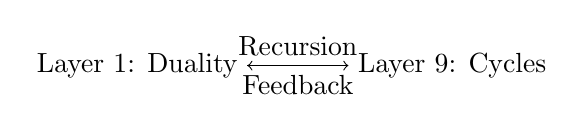
\begin{tikzpicture}
		\node (1) at (0,0) {Layer 1: Duality};
		\node (9) at (4,0) {Layer 9: Cycles};
		\draw[->] (1) -- (9) node[midway,above] {Recursion};
		\draw[->] (9) -- (1) node[midway,below] {Feedback};
	\end{tikzpicture}
	
	\section{Global UBS Enhancements}
	Propose \( \mathcal{UBS}_{total} = \sum_{i=1}^9 \mathcal{UBS}(L_i) + D_f \log_2 (scale) \), where \( D_f \) is the fractal dimension (e.g., 2.5 for quasicrystals) \cite{qgr2023}, unifying scales from Planck to cosmic.
	
	
	\section{Graph Representation and Algorithmic Implementation}
	To operationalize the layered framework and demonstrate its computational viability, we represent it as a dynamic knowledge graph. This graph models the conceptual evolution: nodes represent key concepts and dualities from each layer, while edges denote relationships, transitions, and dualities. The structure is built sequentially, layer by layer, incorporating retroactive cycles in Layer 9 to simulate recursive multiplication and meta-reflection.
	
	The algorithm computes the graph's degree entropy (using Shannon entropy on node degrees) as a proxy for informational complexity, aligning with UBS principles. If entropy exceeds a configurable threshold, an extended ternary search optimizes pruning: removing low-weight edges to approximate an entropy target. This search is enhanced with trigonometric weighting for adaptive midpoints and hyperbolic distances for non-Euclidean spaces, enabling efficient convergence in curved geometries relevant to holographic models.
	
	Key features of the implementation:
	\begin{itemize}
		\item \textbf{Graph Construction}: Nodes and edges are added per layer, with weights representing relational strength. Geometric nodes are positioned in 3D space for visualization.
		\item \textbf{Geometric Iteration}: Functions iteratively build triangles (Layer 4) and tetrahedrons (Layer 5), incorporating fractal scaling (e.g., Sierpinski-like subdivisions).
		\item \textbf{Entropy Calculation}: \( H = -\sum p_i \log_2 p_i \), bounded holographically.
		\item \textbf{Optimization via Extended Ternary Search}: Divides the pruning fraction interval to find an optimal state.
		\item \textbf{Pruning}: Removes low-weight edges to reduce entropy, simulating entropic resolution.
		\item \textbf{Fractal and Code-Theoretic Enhancements}: Iterative fractal expansion (scaling per Axiom 2) and code syntax simulation (per Axiom 6).
		\item \textbf{UBS Integration}: Computes per-layer and global UBS, incorporating fractal dimensions and entropy bounds.
		\item \textbf{Visualizations and Testability}: 3D plots with matplotlib; testable predictions via entropy/UBS thresholds.
	\end{itemize}
	
	The complete, commented source code for this simulation, including fractal geometry generation and UBS computation, is provided as an external file.
	
	\subsection{Simulation Source Code}
	The main simulation is contained in \texttt{lcf\_simulation.py}. This script builds the NetworkX graph, generates fractal geometry, computes entropy, and performs optimization. "These files are available in the accompanying GitHub repository: \url{https://github.com/arturoornelasb/Unified-Holographic-Resonance-Theory-UHRT}."
	
	\begin{center}
		\fcolorbox{black}{gray!10}{%
			\parbox{0.9\textwidth}{%
				\centering\medskip
				\textbf{Referenced File:} \texttt{lcf\_simulation.py} \\
				\small (Contains the core Python simulation script.)
				\medskip
		}}
	\end{center}
	
	\subsection{Example Graph Output}
	The script can generate a GEXF file representing the graph's structure. An example of this output, showing the base 67 nodes and 117 edges, is provided in \texttt{knowledge\_graph\_9\_layers.gexf}.
	
	\begin{center}
		\fcolorbox{black}{gray!10}{%
			\parbox{0.9\textwidth}{%
				\centering\medskip
				\textbf{Referenced File:} \texttt{knowledge\_graph\_9\_layers.gexf} \\
				\small (Contains an example GEXF graph output.)
				\medskip
		}}
	\end{center}
	
	\section{Discussion and Applications}
	
	The Universal Binary Scale (UBS) framework represents a bold attempt to unify disparate measurable concepts under the umbrella of binary information theory. By positing bits as the fundamental unit and emphasizing emergent dualities through iterative duplication, UBS bridges classical and quantum domains while extending to biological and abstract systems. This section discusses the strengths and limitations of the framework and explores potential applications across various fields.
	
	\subsection{Discussion}
	
	One of the primary strengths of UBS lies in its integrative approach, drawing from established principles in information theory to provide a universal metric. For instance, the unification of entropy bounds, as inspired by Bekenstein's work, allows for a consistent representation of phenomena across scales, from Planck units to macroscopic measurements. This aligns with ongoing efforts in physics to reconcile information with thermodynamics, where information theory has been pivotal in understanding emergent phenomena in complex systems. Furthermore, the framework's emphasis on emergent opposites offers a novel lens for duality in nature, such as wave-particle in quantum mechanics or proliferation-apoptosis in biology, potentially simplifying interdisciplinary analyses.
	
	However, UBS is not without limitations. Currently, it remains largely theoretical and speculative, lacking extensive empirical validation or predictive theorems. The formalizations, while mathematically sound, rely on approximations (e.g., discretizing continuums via \( n \to \infty \)) that may not fully capture non-linear or chaotic systems. Critics might argue that reducing all measurables to bits oversimplifies irreducible complexities, similar to debates in applying information theory to Earth sciences where it provides a paradigm but requires careful generalization. Future refinements should address these by deriving testable predictions, such as bounds on biological entropy or quantum computations.
	
	Comparatively, UBS extends ideas from "It from Bit" by Wheeler and Shannon's entropy, but differentiates itself through explicit binary duplication mechanisms. It shares affinities with holographic principles in cosmology and information-theoretic approaches in molecular biology, where entropy measures have quantified sequence complexity. Nonetheless, to gain traction, UBS must demonstrate advantages over existing frameworks like computational biology tools that already leverage information theory for sequence analysis.
	
	\subsection{Applications}
	
	The versatility of UBS opens avenues for applications in multiple domains, leveraging its bit-based unification to model and predict emergent behaviors. In \textbf{physics}, UBS could inform quantum gravity models by quantifying information in black holes or cosmological scales via holographic bounds (Axioma 8). For example, applying \( \mathcal{UBS}(E) \) to energy distributions might predict entropy limits in high-energy physics, building on information theory's role in thermodynamics and AI-inspired physics simulations. This could extend to data-driven model reduction, where information bottlenecks identify predictive variables in complex physical systems.
	
	In \textbf{biology}, the framework's codification of genetic information (Axioma 7) aligns with DNA as binary-like sequences (2 bits per base). UBS might unify mitotic processes and emergent opposites like cell differentiation, aiding in computational biology for gene expression analysis or evolutionary dynamics. Applications could include modeling biological entropy in systems biology, where information theory quantifies network interactions and signaling pathways. Furthermore, mereological decompositions of biomolecules using information measures could reveal functional hierarchies.
	
	In \textbf{artificial intelligence}, UBS's iterative duplication mirrors neural network layers, potentially optimizing models by measuring emergent complexity in bits. This could enhance feature selection and model evaluation, as information theory already underpins machine learning techniques like mutual information for variable dependence. In neurobiology analogs, UBS might model brain information processing, quantifying neural coding efficiency. Broader AI applications include bridging gaps to physics-inspired emergent phenomena, fostering new paradigms in generative models.
	
	Overall, these applications highlight UBS's potential as a foundational tool, warranting further interdisciplinary collaboration and empirical testing to realize its full impact.
	
	
	
	\bibliographystyle{plain}
	\begin{thebibliography}{10}
		
		\bibitem{qgr2023}
		Quantum Gravity Research, Emergence Theory Overview, 2023. \url{https://quantumgravityresearch.org/portfolio/emergence-theory-overview/}
		
		\bibitem{nye2024}
		Nye, L., It From Qubit: Spacetime Emergence from Quantum Entanglement, 2024. \url{https://www.researchgate.net/publication/382146602_It_From_Qubit_Spacetime_Emergence_from_Quantum_Entanglement}
		
		\bibitem{arkani2013}
		Arkani-Hamed, N. and Trnka, J., The Amplituhedron, 2013. \textit{JHEP} 10 (2014) 030. \url{https://arxiv.org/abs/1312.2007}. DOI: 10.1007/JHEP10(2014)030.
		
		\bibitem{verlinde2010}
		Verlinde, E., On the Origin of Gravity and the Laws of Newton, 2010. \textit{JHEP} 04 (2011) 029. \url{https://arxiv.org/abs/1001.0785}. DOI: 10.1007/JHEP04(2011)029.
		
		\bibitem{bekenstein1973}
		Bekenstein, J. D., Black Holes and Entropy, 1973. \textit{Physical Review D} 7(8):2333-2346. \url{https://journals.aps.org/prd/abstract/10.1103/PhysRevD.7.2333}. DOI: 10.1103/PhysRevD.7.2333.
		
		\bibitem{afshordi2019}
		Wolchover, N., How Our Universe Could Emerge as a Hologram, 2019. Quanta Magazine. \url{https://www.quantamagazine.org/how-our-universe-could-emerge-as-a-hologram-20190221/}.
		
		\bibitem{maldacena1999}
		Maldacena, J., The Large N Limit of Superconformal Field Theories and Supergravity, 1999. \textit{Advances in Theoretical and Mathematical Physics} 2:231-252 (1998). \url{https://arxiv.org/abs/hep-th/9711200}. DOI: 10.4310/ATMP.1998.v2.n2.a1.
		
		\bibitem{rovelli1996}
		Rovelli, C., Relational Quantum Mechanics, 1996. \textit{International Journal of Theoretical Physics} 35:1637-1678. \url{https://arxiv.org/abs/quant-ph/9609002}. DOI: 10.1007/BF02302261.
		
		\bibitem{nottale1993}
		Nottale, L., Fractal Space-Time and Microphysics: Towards a Theory of Scale Relativity, 1993. World Scientific. ISBN: 978-981-02-0878-3. DOI: 10.1142/1579.
		
		\bibitem{ashtekar1997}
		Ashtekar, A. and Schilling, T. A., Geometrical Formulation of Quantum Mechanics, 1997. \url{https://arxiv.org/abs/gr-qc/9706069}.
		
		\bibitem{greene1999}
		Greene, B., The Elegant Universe: Superstrings, Hidden Dimensions, and the Quest for the Ultimate Theory, 1999. W.W. Norton. ISBN: 978-0393046884.
		
		\bibitem{bousso2002}
		Bousso, R., The Holographic Principle, 2002. \textit{Reviews of Modern Physics} 74:825-874. \url{https://arxiv.org/abs/hep-th/0203101}. DOI: 10.1103/RevModPhys.74.825.
		
		\bibitem{shannon1948}
		Shannon, C. E., A Mathematical Theory of Communication, 1948. \textit{Bell System Technical Journal} 27:379-423, 623-656. \url{https://ieeexplore.ieee.org/document/6773024}.
		
		\bibitem{wheeler1990}
		Wheeler, J. A., Information, Physics, Quantum: The Search for Links, 1990. In Complexity, Entropy, and the Physics of Information (ed. W. H. Zurek), Addison-Wesley, pp. 3-28.
		
		\bibitem{levine1984}
		Levine, D. and Steinhardt, P. J., Quasicrystals: A new class of ordered structures. \textit{Physical Review Letters} 53(26):2477-2480, 1984. DOI: 10.1103/PhysRevLett.53.2477.
		
		\bibitem{zizzi2000}
		Zizzi, P. A., Quantum computation toward quantum gravity. \textit{arXiv preprint gr-qc/0008049}, 2000. \url{https://arxiv.org/abs/gr-qc/0008049}. Published in \textit{General Relativity and Gravitation} 33:1305-1318 (2001). DOI: 10.1023/A:1012046124033.
		
	\end{thebibliography}
	
\end{document}